% === [ Design ] ===============================================================

\begin{quote}
	``There are two ways of constructing a software design: One way is to make it so simple that there are \textit{obviously} no deficiencies and the other way is to make it so complicated that there are no \textit{obvious} deficiencies. The first method is far more difficult.'' - Tony Hoare, 1980 \cite{hoare_acm_lecture}
\end{quote}

\section{Design}
\label{sec:design}

% TODO: Reformulate to fit the Design section.

% TODO: Add: Separation of concern.

\textbf{NOTE}: \textit{The following paragraph has been moved here from a previous version of the abstract and will therefore feel out of place. The intention is to reformulate it.}

% TODO: Remove note about monolithic decompilers. Focus on the delivering good to the world instead of highlighting all that is bad in the world.

A dynamic approach to problem solving is the composition of independent and specialized components which communicate using well-defined interfaces. Several smaller components may conceptually be arranged in a pipeline of stages which transform, massage or interpret the input in a certain way to solve larger tasks. A well composed pipeline is capable of solving more complex problems than each of its components, problems which may not even have been envisioned by the original component authors. This idea is embodied in the Unix philosophy and it has influenced software construction profoundly. Systems which expose their individual components to end-users facilitate dynamic workflows, as they enable users to adapt and extend each part of the system by adding, removing, replacing or refining components in one or more stages of the pipeline. Meanwhile, the monolithic nature of most production-quality decompilers prevents reverse engineers from utilizing such workflows and may leave them with scripting and plugin support as a substitute.

% TODO: Add design notes
%    - The LLVM IR libraries are developed as reusable components for compilers, decompilers, and other semantic analysis tools. They aim to support generic semantic analysis applications, while satisfying the explicit requirements [1] of the third party llgo compiler.
%
% [1]: https://github.com/go-llvm/llvm/issues/40

% TODO: Add
%   - A decompilation system composed of individual components and based on the principle of separation of concerns.
%   - The system must be language-agnostic so that decompilation passes can be reused from other programming language environments.

foo

% --- [ System Architecture ] --------------------------------------------------

% <howto>
% * the overall structure of the software system (architecture)

% <howto>
% * Software architecture is concerned with deciding what has to be done, and which program component is going to do it (how something is done is left to the detailed design phase, below)
% * It effectively defines the interface between the programs of the system.
% * This stage does not need to consider non-functional requirements (e.g. response time, reliability, maintainability).

\subsection{System Architecture}

% Decompilation Pipeline

% TODO: Describe where the "restructure" component fits in the overall decompilation pipeline. Mention which projects and tools that may be used to fill the gaps. bin_descend and IDA python script of MC-Semantics -> Google Protocol Buffer -> cfg_to_bc -> LLVM IR

% TODO: Rewrite and clarify.

\textbf{NOTE}: \textit{The following paragraph is more of a brain-dump. It is intended to be used as a basis for a future rewrite.}

The decompilation pipeline is made of up several components which are conceptually grouped into three modules. The front-end module translates a variety of inputs (such as binary files and source code) into LLVM IR by utilizing a collection of tools developed by several independent open source projects. The middle-end lifts the LLVM IR to a high-level representation by conducting a control flow analysis which generates a structured CFG of each function. The back-end generates high-level control flow primitives such as if-statements and for-loops based on the structured CFG. In addition it translates the individual instructions of the LLVM IR to expressions and statements of the target programming language (in this case Go). The interaction between the front-end, middle-end and back-end modules is visualized in figure \ref{fig:decompilation_pipeline}.

% * Front-end
%    - binary -> LLVM IR ([MC-Semantics](https://github.com/trailofbits/mcsema), [Dagger](http://dagger.repzret.org/) or [Fracture](https://github.com/draperlaboratory/fracture))
%    - source code -> LLVM IR (clang, ghc, rustc, ...)
% * Middle-end
%    - LLVM IR -> Unstructured CFG ([ll2dot](https://github.com/mewrev/ll2dot))
%    - Unstructured CFG -> Structured CFG ([iso](https://github.com/mewrev/graphs) and [merge](https://github.com/mewrev/graphs).)
%       + Truthfully `ll2go` doesn't make direct use of `iso` or `merge` but rather the graph libraries. A future ambition is to allow `iso` and `merge` to output JSON such that they may be used directly by `ll2go`.
% * Back-end
%    - Structured CFG -> Go ([ll2go](https://github.com/mewrev/ll2go))


\begin{figure}[htbp]
	\begin{center}
		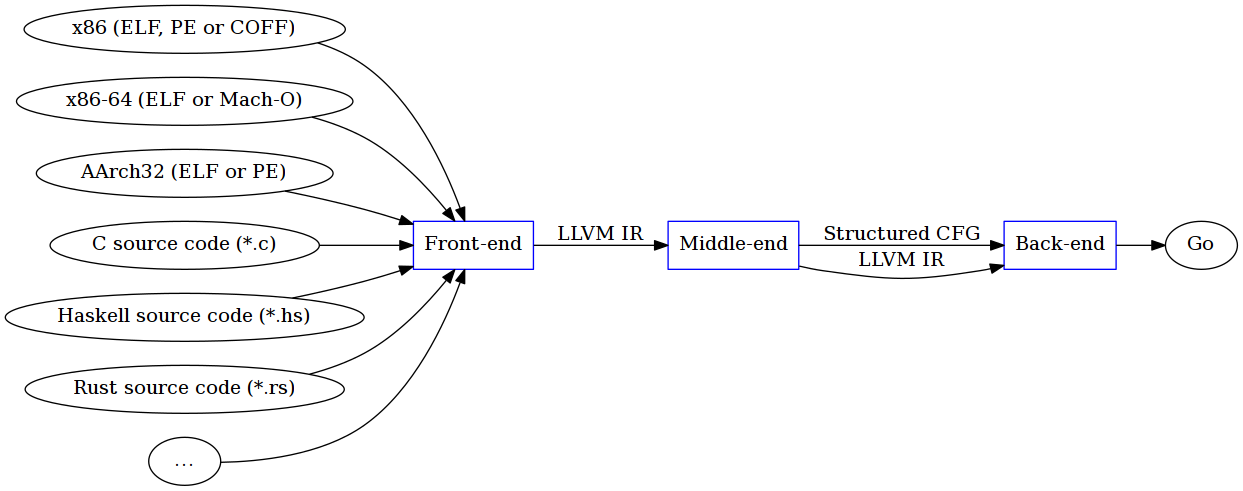
\includegraphics[width=\textwidth]{inc/decompilation_pipeline.png}
		\caption{foo}
		\label{fig:decompilation_pipeline}
	\end{center}
\end{figure}


\subsubsection{Front-end}

% TODO: Rewrite and clarify.

\textbf{NOTE}: \textit{The following paragraph is more of a brain-dump. It is intended to be used as a basis for a future rewrite.}

The front-end module is responsible for converting the input into LLVM IR. Two common scenarios exists, converting binary files (e.g. executables, shared libraries and relocatable object code) and converting source code (e.g. C, Haskell, Rust, …) into LLVM IR. The first scenario is presented in figure \ref{fig:front-end_binary} and the second in figure \ref{fig:front-end_source}.

% TODO: Mention opt --mem2reg.

\begin{figure}[htbp]
	\begin{center}
		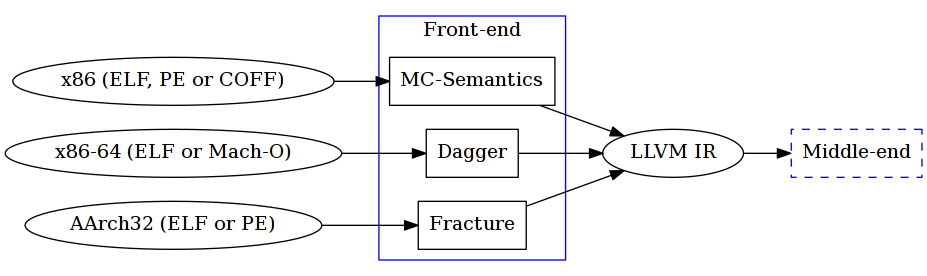
\includegraphics[width=\textwidth]{inc/front-end_binary.png}
		\caption{foo}
		\label{fig:front-end_binary}
	\end{center}
\end{figure}

\begin{figure}[htbp]
	\begin{center}
		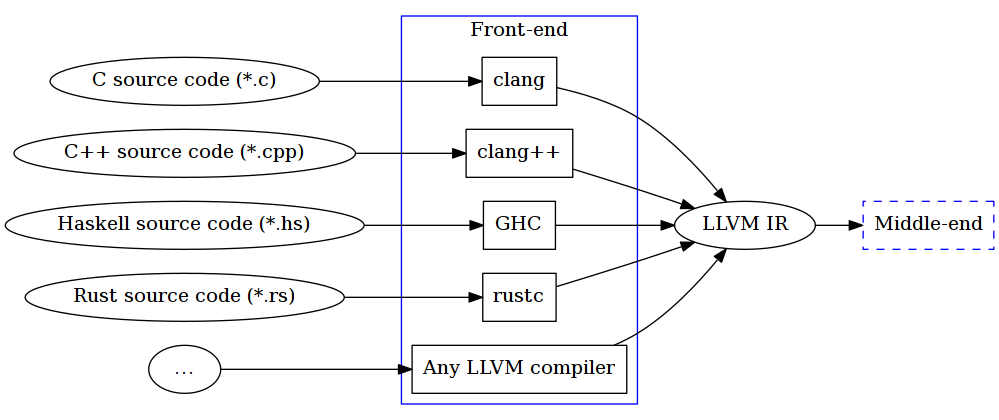
\includegraphics[width=\textwidth]{inc/front-end_source.png}
		\caption{foo}
		\label{fig:front-end_source}
	\end{center}
\end{figure}

\subsubsection{Middle-end}

% TODO: Rewrite and clarify.

% TODO: Create a restructure tool which replaces the use of iso.

\textbf{NOTE}: \textit{The following paragraph is more of a brain-dump. It is intended to be used as a basis for a future rewrite.}

The middle-end is responsible for lifting the LLVM IR to a high-level representation through a series of decompilation passes. The \texttt{ll2dot} tool generates a CFG (in the DOT file format) for each function of a given LLVM IR input file. The \texttt{iso} tool searches for subgraph isomorphisms of control flow primitives in a given CFG. Once located the nodes identified subgraph are merged into a single node which is labeled with the high-level control flow primitive. Successive iterations continue to simplify the CFG until only one node is left, at which point the high-level control flow structure has been recovered. Should the \texttt{iso} tool fail to reduce the graph into a single node, the graph is considered irreducible with regards to the supported high-level control flow primitives. The interaction between the front-end, the \texttt{ll2dot} and \texttt{iso} tools of the middle-end and the back-end is illustrated in figure \ref{fig:middle-end}.

\begin{figure}[htbp]
	\begin{center}
		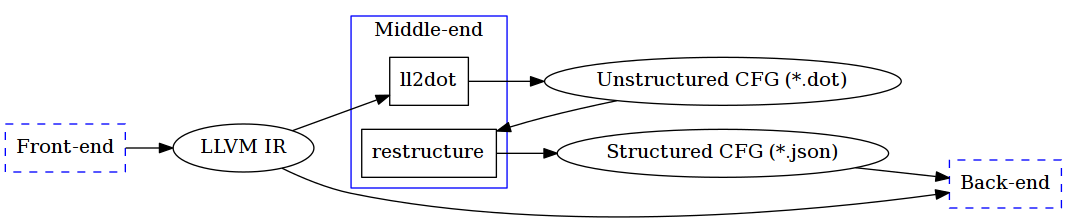
\includegraphics[width=\textwidth]{inc/middle-end.png}
		\caption{foo}
		\label{fig:middle-end}
	\end{center}
\end{figure}

\subsubsection{Back-end}

% TODO: Rewrite and clarify.

% TODO: Add ref to rsc's grind tool.

% TODO: Proof-of-concept. Implement a back-end for another language and written in another language. This would stress test the language-agnostic aspects of the design, thus making sure that the heavy-lifting is done in the middle-end and not in ll2go.

\textbf{NOTE}: \textit{The following paragraph is more of a brain-dump. It is intended to be used as a basis for a future rewrite.}

The back-end is responsible for translating the structured control flow graph of the LLVM IR into a target programming language. The \texttt{ll2go} tool is a proof of concept back-end which produces unpolished Go source code. The polishing is done by separate tools which fixes potential compilation issues and makes the code more idiomatic. The interaction between the middle-end and the back-end is illustrated in figure \ref{fig:back-end}. Currently the \texttt{ll2gofix} replaces return-statements in the \texttt{main} function with calls to \texttt{os.Exit}, which is required since the \texttt{main} function has no return arguments in Go. Instead the Go runtime calls \texttt{os.Exit} with the status-code \texttt{0} once \texttt{main} returns to signal successful termination. This eliminates the need to always end the \texttt{main} function with a \texttt{return 0;} statement as is common practise in C. A future ambition is to make use of and possibly contribute to the \texttt{grind} tool which moves variable declarations closer to their usage, and thus improving readability of the code. Generally the aim is to keep the \texttt{ll2go} tool as simple as possible. The middle-end is responsible for the structural analysis, and as a future ambition the data flow analysis. Since the complexity of the back-end is kept to a minimum it should be trivial to implement support for other output languages.

\begin{figure}[htbp]
	\begin{center}
		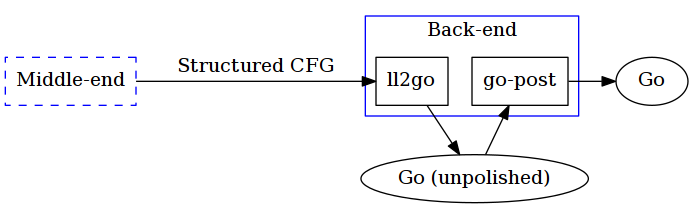
\includegraphics[width=\textwidth]{inc/back-end.png}
		\caption{foo}
		\label{fig:back-end}
	\end{center}
\end{figure}

%%%%%%%%%%%%%%%%%%%%%%%%%%%%%%%%%%%%%%%%%%%%%%%%%%%%%%%%%%%%%%%%%%%%%%%%%%%%%%%%
%%% Component Design %%%%%%%%%%%%%%%%%%%%%%%%%%%%%%%%%%%%%%%%%%%%%%%%%%%%%%%%%%%
%%%%%%%%%%%%%%%%%%%%%%%%%%%%%%%%%%%%%%%%%%%%%%%%%%%%%%%%%%%%%%%%%%%%%%%%%%%%%%%%

% <howto>
% * more detailed design of individual components (design)

% <howto>
% * The intention is that the design should be detailed enough to provide a good guide for actual coding, including details of any particular algorithms to be used.

% TODO: Visualize the dependency graph of the "restructure" tool and describe in detail what input it expects and what output it produces.

% TODO: Write about. Input and output LLVM IR to operate well with components written in other languages. Output LLVM IR with information about high-level control structures stored in the basic block names or in metadata.

% TODO: Mention package division.

% --- [ Control Flow Graph Generation ] ----------------------------------------

\subsection{Control Flow Graph Generation}

foo

% --- [ Control Flow Analysis ] ------------------------------------------------

\subsection{Control Flow Analysis}

% TODO: Add
% * Subgraph Isomorphism Search Algorithm}

foo

\subsubsection{Data-driven Design}

% * Data-driven Design (potential and limitations)
% TODO: Mention: CFG invariants (e.g. single-entry, single-exit)
% TODO: Add notes about the use of DOT-files to describe control flow primitives. Think if and how this could be pushed further to facilitate the development of future back-ends.

foo

\subsubsection{Limitations}

% TODO: Add limitations related to the design choices. Which limitations are easily solvable given more time and which are fundamentally part of the design.
%    - No support for n-way conditionals (e.g.switch-statements).

foo

% --- [ Decompiler Back-end ] --------------------------------------------------

\subsection{Decompiler Back-end}

foo

% TODO: Add
% * Post-processing stages.
